%----------------------------------------------------------------------------------------
% WAT IS EEN FUNCTIE? Alle opgaven zijn eigen werk.
%
% Opbouw: Probleem, Start, leerstof, en op een nieuwe pagina de Opdrachten en Test jezelf (geen Koppel in de 2de graad).
% Labels van dit hoofdstuk beginnen met h1-.
% Verschillen per pakket: alleen in pakket 5 de pijlnotatie f: x -> ..., en in de oefeningenbank een opdracht met
% letters als argument en een functie in stukken. Het leerplan (LPD 17 in pakket 1-3, LPD 21 in 4-5) is in pakket 1-4 gelijk.
%----------------------------------------------------------------------------------------

\mychapter{1}{Wat is een functie?}

\begin{probleem}
\vspace{-1mm}\naast{In parking De Brug hangt dit bord. Ruben parkeert er 3 uur en 10 minuten: hoeveel moet hij betalen? Lies betaalt bij het buitenrijden 7 euro. Hoe lang heeft ze geparkeerd? En kan de parkeerautomaat dat zelf uit de prijs afleiden?}{\begin{tikzpicture}[font=\footnotesize]
  \fill[accent!10] (0,0) rectangle (5.6,2.1);
  \draw[accent,thick] (0,0) rectangle (5.6,2.1);
  \fill[accent,rounded corners=2pt] (.25,.45) rectangle (1.45,1.65);
  \node[text=white,font=\sffamily\bfseries\huge] at (.85,1.05) {P};
  \node[anchor=west,align=left] at (1.65,1.05) {eerste uur: 2 euro\\daarna: 1 euro per\\begonnen halfuur\\maximum 12 euro per dag};
\end{tikzpicture}}
\end{probleem}

\lkr{Leerplan \pakketnaam: LPD \alleenvoor{1,2,3}{17}\alleenvoor{4,5}{21} (wat een functie is, en het verband tussen verwoording, tabel, grafiek en voorschrift), met de wenken: de onafhankelijke en de afhankelijke veranderlijke (het input-outputmodel), een verwoording die de betekenis van het verband uitlegt, en verbanden zonder voorschrift. Ook LPD 1-4 (problemen oplossen en redeneren) komen aan bod. Voorkennis uit de 1ste graad: punten in een assenstelsel, rekenen met formules, rechte evenredigheid. Laat de leerlingen het probleem eerst proberen: de eerste vraag lukt meestal, maar bij de tweede ontdekken ze dat er geen enkel antwoord is. Dat verschil is de kern van het begrip functie.}

Hoe hoger je klimt, hoe kouder het wordt. Hoe langer je belt, hoe meer je betaalt. Overal hangt de ene grootheid af van de andere. In dit hoofdstuk leer je zo'n verband op vier manieren voorstellen: in woorden, in een tabel, in een grafiek en met een formule. Daarna bekijken we wat een functie is: een verband waarbij je altijd hoogstens één antwoord krijgt. Dat begrip gebruik je in de rest van dit boek, en in de jaren die volgen.

\begin{oefeningen}[Start]
\oef{h1-start-1}

\oef{h1-verken}
\end{oefeningen}

%========================================================================================
\section{Verbanden tussen grootheden}

\subsection{Twee veranderlijken}

Hoe snel valt een steen? Je laat een steen vallen van een brug, 80 m boven het water. Hoe hoog hij nog is, hangt af van de tijd die verstreken is sinds je hem losliet. Er zijn dus twee grootheden: de tijd $t$ (in seconden) en de hoogte $h$ (in meter). De tijd kies je zelf: je kijkt na 1 seconde, na 2 seconden, \ldots\ De hoogte volgt daaruit. Dat verschil krijgt een naam.

\begin{theorie}
In een verband tussen twee grootheden is de \textbf{\textcolor{accent}{onafhankelijke veranderlijke}} de grootheid die je zelf kiest. De \textbf{\textcolor{accent}{afhankelijke veranderlijke}} is de grootheid die daaruit volgt.
\end{theorie}

Bij de steen is de tijd $t$ de onafhankelijke veranderlijke en de hoogte $h$ de afhankelijke. Je zegt ook: de hoogte is uitgedrukt \textit{in functie van} de tijd. Meestal noemen we de onafhankelijke veranderlijke $x$ en de afhankelijke $y$.

\voorbeeld{}{De prijs van een taxirit hangt af van de afstand die je rijdt. Welke grootheid is de onafhankelijke veranderlijke, en welke de afhankelijke?\label{vb:h1-veranderlijken}}{%
\uitleg{We vragen ons af: welke grootheid kies je, en welke volgt daaruit?}
De afstand kies je zelf: je zegt waar je heen wilt. De prijs volgt uit de afstand. De afstand is dus de onafhankelijke veranderlijke, de prijs de afhankelijke. Omgekeerd zou ook kunnen (je hebt 20 euro: hoe ver kom je?), maar zo is het verband niet opgesteld.}

\begin{oefeningen}
\oef{h1-veranderlijken}
\end{oefeningen}

\subsection{In woorden en in een tabel}

Natuurkundigen weten hoe ver een steen valt: na $t$ seconden is hij ongeveer $5t^2$ meter gevallen (als we de luchtweerstand verwaarlozen). Dat is een \textit{verwoording} van het verband. Ze is kort, maar je ziet er niet meteen in hoe hoog de steen na 3 seconden is. Een \textit{tabel} toont dat beter.

\voorbeeld{}{Maak een tabel met de hoogte van de steen na 0, 1, 2, 3 en 4 seconden.\label{vb:h1-tabel}}{%
\uitleg{Per tijdstip rekenen we uit hoe ver de steen gevallen is, en trekken dat af van 80 m.}
\begin{stappen}
t = 2: \quad 5 \cdot 2^2 = 5 \cdot 4 = 20 & Na 2 seconden is hij 20 m gevallen. \\
h = 80 - 20 = 60 & Hij is dan nog 60 m hoog.
\end{stappen}
Zo vind je ook de andere hoogtes:

\vspace{1mm}
\waardetabel[$t$ (s)][$h$ (m)]{5}{0 & 1 & 2 & 3 & 4}{80 & 75 & 60 & 35 & 0}

\vspace{1mm}
Na 4 seconden is de hoogte 0: de steen raakt het water.}

Een tabel is handig om waarden op te zoeken, maar ze toont alleen de waarden die erin staan. Hoe hoog is de steen na $2\tfrac12$ seconde? Dat staat niet in de tabel.

\subsection{In een grafiek}

Een grafiek toont het hele verloop in één beeld. Zet de onafhankelijke veranderlijke op de horizontale as en de afhankelijke op de verticale as. Elk koppel uit de tabel wordt een punt: $(0, 80)$, $(1, 75)$, $(2, 60)$, enzovoort. De tijd loopt ononderbroken door, dus tussen twee punten zijn er nog veel meer tijdstippen. We verbinden de punten daarom met een vloeiende lijn.

\naast{\begin{stappenvrij}{3.4cm}{4.7cm}
(0, 80),\ (1, 75) & Elk koppel uit de tabel is een punt. \\
(2, 60),\ (3, 35) & De punten liggen niet op een rechte: de steen valt steeds sneller. \\
(4, 0) & Daar raakt de steen het water.
\end{stappenvrij}

\vspace{2mm}
Nu kun je ook aflezen wat niet in de tabel stond. De stippellijn toont dat de steen na $2\tfrac12$ seconde ongeveer 49 m hoog is. Uit de verwoording volgt precies: $5 \cdot 2,5^2 = 31,25$, dus $80 - 31,25 = 48,75$ m. Een grafiek geeft dus snel een goede schatting, maar zelden een exacte waarde.}{\begin{tikzpicture}[x=1.2cm,y=.045cm]
  \roosterleeg[$t$ (s)][$h$ (m)]{0}{0.5}{4.5}{0}{10}{90}
  \xgetallen{1,2,3,4}
  \ygetallen{20,40,60,80}
  \oorsprong
  \kromme{0}{4}{80-5*(\x)^2}
  \foreach \t in {0,1,2,3,4}{\punt{\t}{80-5*\t*\t}}
  \aflezen{2.5}{48.75}
\end{tikzpicture}}

\voorbeeld{}{Lees op de grafiek af wanneer de steen 40 m hoog is.\label{vb:h1-grafiek}}{%
\naast{\uitleg{Nu ken je de hoogte, en zoek je de tijd. We vertrekken op de verticale as.}
\begin{stappenvrij}{2.6cm}{5.4cm}
h = 40 & Vertrek bij 40 op de verticale as. \\
& Ga horizontaal tot je de grafiek raakt. \\
t \approx 2,8 & Ga verticaal naar beneden en lees af.
\end{stappenvrij}
Na ongeveer 2,8 seconden is de steen 40 m hoog.}{\begin{tikzpicture}[x=.9cm,y=.032cm]
  \roosterleeg[$t$][$h$]{0}{0.5}{4.5}{0}{10}{90}
  \xgetallen{1,2,3,4}
  \ygetallen{20,40,60,80}
  \kromme{0}{4}{80-5*(\x)^2}
  \draw[grijs,dashed,->] (0,40) -- (2.83,40) -- (2.83,0);
  \punt{2.83}{40}
\end{tikzpicture}}}

\begin{oefeningen}
\oef{h1-grafiek}
\end{oefeningen}

\subsection{Met een formule}

De verwoording ``na $t$ seconden is de steen $5t^2$ meter gevallen'' kun je ook in symbolen schrijven. De hoogte is 80 min wat hij gevallen is:
\[h = 80 - 5t^2.\]
Zo'n formule noemen we een \textit{voorschrift}. Met een voorschrift reken je elke waarde exact uit, ook voor tijdstippen die niet in de tabel staan.

\voorbeeld{}{Bereken met het voorschrift $h = 80 - 5t^2$ hoe hoog de steen na $1,5$ seconde is.\label{vb:h1-formule}}{%
\uitleg{We vullen $t = 1,5$ in. De macht gaat voor de vermenigvuldiging, en die gaat voor de aftrekking.}
\begin{stappen}
h = 80 - 5 \cdot 1,5^2 & Vul $1,5$ in voor $t$. \\
= 80 - 5 \cdot 2,25 & Eerst de macht: $1,5^2 = 2,25$. \\
= 80 - 11,25 = 68,75 & Dan vermenigvuldigen en aftrekken.
\end{stappen}
Na $1,5$ seconde is de steen $68,75$ m hoog. Op de grafiek ligt het punt $(1,5;\ 68,75)$ tussen $(1, 75)$ en $(2, 60)$, zoals verwacht.}

We hebben nu vier voorstellingen van hetzelfde verband. Elk heeft haar sterkte: de verwoording vertelt wat er gebeurt, de tabel geeft waarden om op te zoeken, de grafiek toont het verloop en het voorschrift geeft exacte waarden.

Niet elk verband heeft een voorschrift. De temperatuur op een dag, de waterstand in een haven of je hartslag tijdens het sporten ken je alleen uit metingen: uit een tabel of een grafiek. Een formule die ze exact geeft, bestaat niet. Toch kun je er vragen over beantwoorden, zoals je in hoofdstuk 3 zult zien.

\begin{oefeningen}
\oef{h1-formule}
\end{oefeningen}

%========================================================================================
\section{Wat is een functie?}

\subsection{Hoogstens één antwoord}

Een bioscoopticket kost 8 euro voor wie jonger is dan 12 jaar, en 12 euro vanaf 12 jaar. Bij elke leeftijd hoort precies één prijs: de kassa kan die prijs altijd uitrekenen. Maar omgekeerd lukt het niet. Wie 8 euro betaalt, kan 5 jaar oud zijn, of 9 jaar. Bij één prijs horen veel leeftijden.

Zo'n verschil is belangrijk. Een verband waarbij je bij elke keuze hoogstens één antwoord krijgt, is voorspelbaar: geef de waarde van $x$, en de waarde van $y$ ligt vast. Dat soort verband krijgt een naam.

\begin{theorie}
Een verband tussen $x$ en $y$ is een \textbf{\textcolor{accent}{functie}} als bij elke waarde van $x$ hoogstens één waarde van $y$ hoort.
\end{theorie}

Waarom ``hoogstens één'' en niet ``precies één''? Soms hoort er bij een waarde van $x$ geen $y$: de steen heeft geen hoogte na $-3$ seconden. Dat mag. Wat niet mag, is dat er bij één $x$ twee verschillende waarden van $y$ horen. De ticketprijs is dus een functie van de leeftijd, maar de leeftijd is geen functie van de ticketprijs.

\voorbeeld{}{Is $y$ een functie van $x$ in deze tabel? \quad \waardetabel[$x$][$y$]{6}{1 & 2 & 3 & 3 & 4 & 5}{4 & 6 & 7 & 9 & 9 & 10}\label{vb:h1-tabelfunctie}}{%
\uitleg{We zoeken een waarde van $x$ die twee keer voorkomt, met een andere waarde van $y$.}
Bij $x = 3$ horen twee waarden: $y = 7$ en $y = 9$. Dit verband is dus \textit{geen} functie. Dat $y = 9$ zowel bij $x = 3$ als bij $x = 4$ hoort, is geen probleem: twee waarden van $x$ mogen dezelfde $y$ hebben.}

\voorbeeld{}{Bij elke leerling van een klas hoort zijn of haar geboortemaand. Is de geboortemaand een functie van de leerling? En is de leerling een functie van de geboortemaand?\label{vb:h1-woordenfunctie}}{%
\uitleg{We kijken telkens of er bij één keuze twee antwoorden kunnen horen.}
Elke leerling heeft precies één geboortemaand: de geboortemaand is een functie van de leerling. Maar in een maand kunnen meerdere leerlingen jarig zijn, bijvoorbeeld Emma en Yusuf in maart. Bij maart horen dan twee leerlingen: de leerling is geen functie van de geboortemaand.}

\begin{oefeningen}
\oef{h1-functieofniet}
\end{oefeningen}

\subsection{De notatie \texorpdfstring{$f(x)$}{f(x)}}

Een functie krijgt meestal een letter als naam, zoals $f$, $g$ of $h$. De waarde van $y$ die bij een waarde van $x$ hoort, schrijven we kort als $f(x)$, en we lezen dat als ``$f$ van $x$''. Bij de steen is de hoogte een functie van de tijd: $h(t) = 80 - 5t^2$, en $h(2) = 60$ betekent dat de steen na 2 seconden 60 m hoog is. Je kunt een functie zien als een machine: je stopt er een getal $x$ in (de input), en er komt hoogstens één getal $f(x)$ uit (de output).

\begin{theorie}
Bij een functie $f$ is $\formule{f(x)}$ de \textbf{\textcolor{accent}{functiewaarde}} van $x$: de waarde van $y$ die bij $x$ hoort. We schrijven $\formule{y = f(x)}$.

\vspace{1mm}
Het \textbf{\textcolor{accent}{voorschrift}} van $f$ zegt hoe je $f(x)$ berekent, bijvoorbeeld $f(x) = 3x - 4$.
\end{theorie}

Let op: $f(x)$ is geen vermenigvuldiging. Het is één symbool, net zoals een huisnummer bij een straat hoort. In plaats van functiewaarde zeggen we ook \textit{beeld}: 2 is het beeld van 3 als $f(3) = 2$.

\begin{alleenvoor}{5}
Je ziet ook de notatie $f: x \mapsto 3x - 4$, met een pijl met een streepje. Lees die als ``$f$ beeldt $x$ af op $3x - 4$''. Ze zegt hetzelfde als $f(x) = 3x - 4$.
\end{alleenvoor}

\voorbeeld{}{Gegeven: $f(x) = 3x - 4$. Bereken $f(2)$ en $f(-1)$.\label{vb:h1-functiewaarde}}{%
\uitleg{We vervangen $x$ overal door het getal tussen de haakjes. Een negatief getal zetten we zelf tussen haakjes, zodat het minteken niet verloren gaat.}
\begin{stappen}
f(2) = 3 \cdot 2 - 4 = 6 - 4 = 2 & Vul 2 in voor $x$. \\
f(-1) = 3 \cdot (-1) - 4 = -3 - 4 = -7 & Vul $-1$ in, tussen haakjes.
\end{stappen}}

\voorbeeld{}{Gegeven: $g(x) = x^2 - 2x$. Bereken $g(-3)$.\label{vb:h1-functiewaarde2}}{%
\uitleg{Ook hier zetten we $-3$ tussen haakjes. Zo zie je dat het kwadraat van $-3$ positief is.}
\begin{stappen}
g(-3) = (-3)^2 - 2 \cdot (-3) & Vervang beide keren $x$ door $(-3)$. \\
= 9 + 6 = 15 & $(-3)^2 = 9$ en $-2 \cdot (-3) = +6$.
\end{stappen}}

\begin{werkwijze}
Vervang in het voorschrift elke $x$ door het gegeven getal, met een negatief getal tussen haakjes. Reken daarna uit in de gewone volgorde: haakjes, machten, vermenigvuldigen en delen, optellen en aftrekken.
\end{werkwijze}

\nujij{Gegeven: $f(x) = 5 - 2x$. Bereken $f(0)$, $f(4)$ en $f(-3)$.}{$f(0) = 5$, $f(4) = -3$, $f(-3) = 11$.}

\begin{oefeningen}
\oef{h1-functiewaarde}
\end{oefeningen}

\subsection{De grafiek van een functie}

De grafiek van een functie $f$ bestaat uit alle punten $(x, f(x))$. Kun je aan een kromme zien of ze de grafiek van een functie is? Denk aan de definitie: bij één waarde van $x$ mag hoogstens één $y$ horen. Twee punten van de kromme met dezelfde $x$ maar een andere $y$ liggen recht boven elkaar, op dezelfde verticale rechte. Dat mag dus niet.

\begin{theorie}
\begin{stelling}{Verticale rechten}
Een kromme is de grafiek van een functie als elke verticale rechte de kromme hoogstens één keer snijdt.
\end{stelling}
\end{theorie}

\voorbeeld{}{Welke van deze krommen zijn de grafiek van een functie?\label{vb:h1-verticaal}}{%
\figuren{\begin{tikzpicture}[x=.42cm,y=.42cm]
  \roosterleeg{-3}{1}{3}{-3}{1}{3}
  \doorpunten{(-3,-2) (-2,1) (-1,2) (0,1) (1,-1) (2,-1.5) (3,1)}
  \draw[hulplijn] (1,-3) -- (1,3);
  \node[font=\footnotesize] at (0,-3.9) {1};
\end{tikzpicture}\qquad
\begin{tikzpicture}[x=.42cm,y=.42cm]
  \roosterleeg{-3}{1}{3}{-3}{1}{3}
  \draw[accent,thick] (0,0) circle (2.2);
  \draw[hulplijn] (1,-3) -- (1,3);
  \punt{1}{1.96}\punt{1}{-1.96}
  \node[font=\footnotesize] at (0,-3.9) {2};
\end{tikzpicture}\qquad
\begin{tikzpicture}[x=.42cm,y=.42cm]
  \roosterleeg{-3}{1}{3}{-3}{1}{3}
  \draw[accent,thick] plot[domain=-1.7:1.7,samples=40,smooth] ({(\x)^2-2},\x);
  \draw[hulplijn] (-1,-3) -- (-1,3);
  \punt{-1}{1}\punt{-1}{-1}
  \node[font=\footnotesize] at (0,-3.9) {3};
\end{tikzpicture}\qquad
\begin{tikzpicture}[x=.42cm,y=.42cm]
  \roosterleeg{-3}{1}{3}{-3}{1}{3}
  \draw[accent,thick] (-3,1) -- (0,1);
  \draw[accent,thick] (0,-1) -- (3,-1);
  \punt{0}{1}\openpunt{0}{-1}
  \node[font=\footnotesize] at (0,-3.9) {4};
\end{tikzpicture}}
\uitleg{We schuiven in gedachten een verticale rechte over elke figuur, en kijken of ze ergens twee punten raakt.}
\begin{stappen}
\text{Kromme 1: functie} & De kromme stijgt en daalt, maar elke verticale rechte snijdt haar één keer. \\
\text{Kromme 2: geen functie} & De rechte $x = 1$ snijdt de cirkel twee keer. \\
\text{Kromme 3: geen functie} & De rechte $x = -1$ snijdt de kromme twee keer. \\
\text{Kromme 4: functie} & Bij $x = 0$ hoort alleen het volle bolletje: het open bolletje hoort er niet bij.
\end{stappen}}

Een kromme die stijgt en daalt, kan dus best de grafiek van een functie zijn. Het gaat er alleen om dat ze nergens recht boven zichzelf ligt.

\begin{oefeningen}
\oef{h1-verticaal}
\end{oefeningen}

\subsection{Functiewaarden aflezen}

Op een grafiek kun je in twee richtingen lezen. Ken je $x$, dan zoek je $f(x)$: ga verticaal naar de grafiek en dan horizontaal naar de $y$-as. Ken je de functiewaarde, dan zoek je de $x$-waarden die erbij horen: ga horizontaal vanaf de $y$-as naar de grafiek, en dan verticaal naar de $x$-as. In de tweede richting kun je meer dan één antwoord vinden. Dat is geen tegenspraak met de definitie van een functie: verschillende $x$-waarden mogen dezelfde functiewaarde hebben.

\voorbeeld{}{Hiernaast staat de grafiek van een functie $f$. Lees af: $f(-1)$ en $f(2)$. Voor welke waarden van $x$ is $f(x) = 2$?\label{vb:h1-aflezen}}{%
\naast{\uitleg{Voor $f(-1)$ vertrekken we op de $x$-as. Voor $f(x) = 2$ vertrekken we op de $y$-as, bij 2, en zoeken we alle punten van de grafiek op die hoogte.}
\begin{stappenvrij}{2.4cm}{5.2cm}
f(-1) = 3 & Boven $x = -1$ ligt de grafiek op hoogte 3. \\
f(2) = -1 & Onder $x = 2$ ligt de grafiek op hoogte $-1$. \\
x = -2,\ 0 \text{ of } 4 & De horizontale rechte op hoogte 2 snijdt de grafiek in drie punten.
\end{stappenvrij}}{\begin{tikzpicture}[x=.5cm,y=.5cm]
  \rooster{-4}{1}{5}{-2}{1}{4}
  \doorpunten{(-3,-1) (-2,2) (-1,3) (0,2) (1,0) (2,-1) (3,0) (4,2) (4.4,3.2)}
  \draw[hulplijn] (-4,2) -- (5,2);
  \foreach \t in {-2,0,4}{\punt{\t}{2}}
  \aflezen{-1}{3}
  \punt{-1}{3}
\end{tikzpicture}}}

\begin{oefeningen}
\oef{h1-aflezen}
\end{oefeningen}

%========================================================================================
\section{Van de ene voorstelling naar de andere}

\subsection{Van voorschrift naar tabel en grafiek}

Hoe ziet de grafiek van $f(x) = x^2 - 2x - 1$ eruit? Uit het voorschrift alleen zie je dat niet. Maak daarom eerst een tabel, en teken dan de punten.

\voorbeeld{}{Teken de grafiek van $f(x) = x^2 - 2x - 1$ voor $x$ van $-1$ tot $3$.\label{vb:h1-tekenen}}{%
\naast{\uitleg{We kiezen gehele waarden van $x$ van $-1$ tot 3, rekenen de functiewaarden uit en zetten de punten in een assenstelsel.}
\begin{stappenvrij}{3.9cm}{3.4cm}
f(-1) = 1 + 2 - 1 = 2 & $(-1)^2 = 1$ en $-2 \cdot (-1) = 2$. \\
f(0) = -1 & Alleen $-1$ blijft over. \\
f(1) = 1 - 2 - 1 = -2 & \\
f(2) = 4 - 4 - 1 = -1 & \\
f(3) = 9 - 6 - 1 = 2 &
\end{stappenvrij}

\vspace{1mm}
\waardetabel{5}{-1 & 0 & 1 & 2 & 3}{2 & -1 & -2 & -1 & 2}

\vspace{1mm}
De punten liggen niet op een rechte. We verbinden ze met een vloeiende, gebogen lijn, en niet met rechte stukjes.}{\begin{tikzpicture}[x=.6cm,y=.6cm]
  \rooster{-2}{1}{4}{-3}{1}{3}
  \kromme{-1.3}{3.3}{(\x)^2-2*(\x)-1}
  \foreach \t in {-1,0,1,2,3}{\punt{\t}{\t*\t-2*\t-1}}
\end{tikzpicture}}}

\begin{werkwijze}
Kies een paar waarden van $x$, gelijkmatig verdeeld. Bereken de functiewaarden en zet ze in een tabel. Teken de punten $(x, f(x))$ en verbind ze met een vloeiende lijn. Twijfel je over het verloop tussen twee punten, bereken dan een extra functiewaarde.
\end{werkwijze}

\begin{oefeningen}
\oef{h1-tekenen}
\end{oefeningen}

\subsection{Van verwoording naar voorschrift}

In een situatie uit het dagelijks leven staat het voorschrift er meestal niet bij. Je stelt het zelf op. Begin met een paar getallen: wat gebeurt er bij 1, bij 2, bij 10? Zo zie je welke bewerkingen je doet, en die schrijf je daarna met een letter.

\voorbeeld{}{Een fotodienst rekent $0,25$ euro per afdruk en 3 euro verzendkosten per bestelling. Stel een voorschrift op voor de prijs $p$ (in euro) van een bestelling van $n$ foto's.\label{vb:h1-voorschrift}}{%
\uitleg{We rekenen eerst een paar bestellingen uit, en zoeken wat telkens terugkomt.}
\begin{stappen}
10 \text{ foto's:}\ 0,25 \cdot 10 + 3 = 5,50 & De afdrukken, plus de verzendkosten. \\
40 \text{ foto's:}\ 0,25 \cdot 40 + 3 = 13 & Hetzelfde patroon, met 40. \\
p(n) = 0,25\,n + 3 & Het aantal foto's wordt de letter $n$.
\end{stappen}}

Kan $n$ hier elk getal zijn? Nee: je bestelt geen $2,5$ foto's of $-3$ foto's. Alleen natuurlijke getallen hebben zin. Hoe je dat in een grafiek toont, zie je in het volgende onderdeel.

\voorbeeld{}{Een rechthoek heeft een omtrek van 20 cm. Druk de oppervlakte $A$ uit in functie van de breedte $x$ (in cm).\label{vb:h1-rechthoek}}{%
\naast{\uitleg{We proberen eerst een rechthoek met een breedte van 3 cm. De breedte en de lengte samen zijn de helft van de omtrek: $20 : 2 = 10$ cm. Daarna doen we hetzelfde met $x$.}}{\begin{tikzpicture}[scale=.36,font=\scriptsize]
  \fill[accent!15] (0,0) rectangle (7,3);
  \draw[accent,thick] (0,0) rectangle (7,3);
  \node[left] at (0,1.5) {$x$};
  \node[below] at (3.5,0) {$10 - x$};
  \node at (3.5,1.5) {$A$};
\end{tikzpicture}}
\begin{stappen}
\text{breedte } 3:\ \text{lengte } 10 - 3 = 7 & Breedte plus lengte is 10. \\
A = 3 \cdot 7 = 21 & Oppervlakte: breedte maal lengte. \\
\text{breedte } x:\ \text{lengte } 10 - x & Hetzelfde, met $x$ in plaats van 3. \\
A(x) = x\,(10 - x) & Breedte maal lengte.
\end{stappen}
De breedte ligt tussen 0 en 10 cm, anders is er geen rechthoek. Een tabel toont dat de oppervlakte eerst groeit en dan weer kleiner wordt: $A(1) = 9$, $A(3) = 21$, $A(5) = 25$, $A(7) = 21$, $A(9) = 9$. Het vierkant van 5 bij 5 heeft de grootste oppervlakte.}

\begin{oefeningen}
\oef{h1-voorschrift}
\end{oefeningen}

\subsection{Losse punten of een doorlopende lijn}

Mag je de punten van een grafiek altijd verbinden? Bij de steen wel: de tijd loopt ononderbroken door, en op elk tijdstip heeft de steen een hoogte. Bij de foto's niet: tussen 10 en 11 foto's ligt geen enkele bestelling. De grafiek bestaat dan uit losse punten.

\voorbeeld{}{Teken de grafiek van de prijs $p(n) = 0,25\,n + 3$ voor bestellingen van 0 tot 8 foto's.\label{vb:h1-losse}}{%
\naast{\uitleg{Alleen natuurlijke getallen hebben zin voor $n$. We rekenen de prijzen uit en tekenen de punten, zonder ze te verbinden.}
\waardetabel[$n$][$p(n)$]{5}{0 & 2 & 4 & 6 & 8}{3 & 3,5 & 4 & 4,5 & 5}

\vspace{1mm}
De punten liggen op een rechte, maar de rechte zelf is niet de grafiek: een bestelling van $2,5$ foto's bestaat niet. Bij $n = 0$ bestel je niets. Of je dan 3 euro betaalt, hangt af van de fotodienst: het voorschrift geldt eigenlijk pas vanaf één foto.}{\begin{tikzpicture}[x=.55cm,y=.55cm]
  \roosterleeg[$n$][$p$]{0}{1}{8}{0}{1}{5}
  \xgetallen{2,4,6,8}\ygetallen{1,2,3,4,5}\oorsprong
  \foreach \n in {0,...,8}{\punt{\n}{.25*\n+3}}
\end{tikzpicture}}}

\subsection{Van grafiek naar verwoording}

Een grafiek vertelt een verhaal. Om het te lezen, kijk je naar de stukken: waar stijgt de grafiek, waar is ze horizontaal, waar daalt ze? Hoe steiler een stuk, hoe sneller de afhankelijke veranderlijke verandert.

\voorbeeld{}{Nora wandelt naar het huis van een vriendin en terug. De grafiek toont haar afstand $d$ tot thuis (in km) in functie van de tijd $t$ (in minuten). Beschrijf de wandeling in woorden.\label{vb:h1-verhaal}}{%
\naast{\uitleg{We lezen de grafiek stuk per stuk, van links naar rechts.}
\begin{stappenvrij}{1.6cm}{5.2cm}
0 \text{ tot } 20 & De afstand stijgt van 0 tot 2 km: Nora wandelt van huis weg, 2 km in 20 minuten. \\
20 \text{ tot } 50 & De afstand blijft 2 km: ze is bij haar vriendin, een halfuur lang. \\
50 \text{ tot } 60 & De afstand daalt van 2 tot 0 km in 10 minuten: ze gaat terug, twee keer zo snel als op de heenweg. Dat zie je aan het steilere stuk.
\end{stappenvrij}}{\begin{tikzpicture}[x=.09cm,y=.75cm]
  \roosterleeg[$t$][$d$]{0}{10}{70}{0}{0.5}{2.5}
  \xgetallen{20,40,60}\ygetallen{1,2}\oorsprong
  \gebroken{(0,0) (20,2) (50,2) (60,0)}
\end{tikzpicture}}}

\begin{oefeningen}
\oef{h1-verhaal}
\end{oefeningen}

\voorbeeld{}{Terug naar het probleem. In parking De Brug hangt een bord: het eerste uur kost 2 euro, daarna betaal je 1 euro per begonnen halfuur, met een maximum van 12 euro per dag. Ruben parkeert er 3 uur en 10 minuten: hoeveel moet hij betalen? Lies betaalt bij het buitenrijden 7 euro. Hoe lang heeft ze geparkeerd? En kan de parkeerautomaat dat zelf uit de prijs afleiden?\label{vb:h1-terug}}{%
\uitleg{We maken een tabel met de prijs per tijdsvak, en tekenen de grafiek. Een parkeerduur op de grens van twee vakken, zoals precies 3 uur, hoort nog bij het goedkopere vak: het volgende halfuur is dan nog niet begonnen.}
{\small\waardetabel[duur (h)][prijs (\eur)]{8}{\ivog{0}{1} & \ivog{1}{1,5} & \ivog{1,5}{2} & \ivog{2}{2,5} & \ivog{2,5}{3} & \ivog{3}{3,5} & \ldots & \text{na } 5,5}{2 & 3 & 4 & 5 & 6 & 7 & \ldots & 12}}

\vspace{1mm}
\naast{\begin{stappenvrij}{2cm}{3.6cm}
3 \text{ h } 10 \text{ min} & Ligt tussen 3 h en 3 h 30 min. \\
\text{prijs } 7 \text{ euro} & Het zesde vak in de tabel.
\end{stappenvrij}

\vspace{1mm}
Ruben betaalt 7 euro. Bij 7 euro hoort in de grafiek een heel stuk: elke duur na 3 uur en tot en met 3 uur en 30 minuten. Lies heeft dus langer dan 3 uur geparkeerd, en hoogstens 3 uur en een half. Preciezer kan het niet: de automaat kan de parkeerduur niet uit de prijs afleiden. De prijs is een functie van de parkeerduur, maar de parkeerduur is geen functie van de prijs.

\vspace{1mm}
In de grafiek tonen de bolletjes wat bij elk stuk hoort: een vol bolletje hoort erbij, een open bolletje niet. De punten van de grafiek verbinden we niet verticaal, want dan zou er bij precies 3 uur een hele reeks prijzen horen.}{\begin{tikzpicture}[x=1.05cm,y=.32cm]
  \roosterleeg[$t$ (h)][prijs]{0}{0.5}{6.5}{0}{1}{13}
  \xgetallen{1,2,3,4,5,6}\ygetallen{2,4,6,8,10,12}\oorsprong
  \draw[hulplijn] (0,7) -- (6.5,7);
  \draw[accent,thick] (0,2) -- (1,2); \openpunt{0}{2}\punt{1}{2}
  \foreach \k in {1,...,9}{%
    \draw[accent,thick] ({1+(\k-1)/2},{2+\k}) -- ({1+\k/2},{2+\k});
    \openpunt{1+(\k-1)/2}{2+\k}\punt{1+\k/2}{2+\k}}
  \draw[accent,thick] (5.5,12) -- (6.5,12); \openpunt{5.5}{12}
  \asdeel{3}{3.5}
\end{tikzpicture}}}

%========================================================================================
\opdrachtenkop

\begin{oefeningen}
\oef{h1-o1}

\oef{h1-o3}

\oef{h1-o2}

\oef{h1-o6}

\needspace{14\baselineskip}
\oef{h1-o4}

\oef{h1-o8}

\oef{h1-o7}

\oef{h1-o9}

\oef{h1-o5}

\oef{h1-o11}

\oef{h1-o10}

\oef{h1-o12}

\oef{h1-o18}

\oef{h1-o13}

\oef{h1-o15}

\needspace{16\baselineskip}
\oef{h1-o14}

\oef{h1-o16}

\oef{h1-o19}

\oef{h1-o17}

\oef{h1-o20}

\oef{h1-o21}

\oef{h1-o22}

\oef{h1-o23}

\oef{h1-o24}

\oef{h1-o25}
\end{oefeningen}

%----------------------------------------------------------------------------------------
\opdrachtsectie{Test jezelf}

\begin{oefeningen}
\oef{h1-t1}

\oef{h1-t2}

\needspace{6\baselineskip}
\oef{h1-t3}

\oef{h1-t4}

\oef{h1-t5}

\oef{h1-t6}

\oef{h1-t7}
\end{oefeningen}

\herhaalschema{%
  \fv{oef:h1-t1}{vb:h1-veranderlijken}{oef:h1-veranderlijken}%
  \fv{oef:h1-t2}{vb:h1-tabelfunctie}{oef:h1-functieofniet}%
  \fv{oef:h1-t3}{vb:h1-functiewaarde2}{oef:h1-functiewaarde}%
  \fv{oef:h1-t4}{vb:h1-verticaal}{oef:h1-verticaal}%
  \fv{oef:h1-t5}{vb:h1-aflezen}{oef:h1-aflezen}%
  \fv{oef:h1-t6}{vb:h1-tekenen}{oef:h1-tekenen}%
  \fv{oef:h1-t7}{vb:h1-voorschrift}{oef:h1-voorschrift}}

\ifzelfstudie
\section*{Maak je eigen samenvatting}
Sluit dit boek en schrijf in je schrift: wat de onafhankelijke en de afhankelijke veranderlijke zijn, de vier voorstellingen van een verband met een voorbeeld, wat een functie is, wat $f(x)$ betekent, hoe je aan een grafiek ziet of ze bij een functie hoort, en wanneer je de punten van een grafiek verbindt. Vergelijk daarna met de kaders.
\fi
